\documentclass[a4paper]{article}
\usepackage[utf8]{inputenc}
\usepackage[russian,english]{babel}
\usepackage[T2A]{fontenc}
\usepackage[left=10mm, top=20mm, right=18mm, bottom=15mm, footskip=10mm]{geometry}
\usepackage{indentfirst}
\usepackage{amsmath,amssymb}
\usepackage[italicdiff]{physics}
\usepackage{graphicx}
\graphicspath{{images/}}
\DeclareGraphicsExtensions{.pdf,.png,.jpg}
\usepackage{wrapfig}

\usepackage{caption}
\captionsetup[figure]{name=Рисунок}
\captionsetup[table]{name=Таблица}
  
\title{\underline{Отчет о выполненой лабораторной работе 1.4.5}}
\author{Антон Хмельницкий, Б01-306}


\begin{document}

\maketitle
\begin{center}\textbf{Изучение колебаний струны}\end{center}

\section{Аннотация}
\underline{Цель работы}: 
Изучить поперечные стоячие волн на тонкой натянутой струне; измерить собственные частоты колебаний струны и проверить условие образования стоячих волн; измерить скорость распространения поперечных волн на струне и исследовать её зависимость от натяжения струны.

\underline{Оборудование}: 
В работе используются: закрепленная на станине стальная струна, набор грузов, электромагнитные датчики, звуковой генератор, двухканальный осциллограф, частотомер.

\section{Теоретические сведения}\par

Струной в акустике называют однородную тонкую гибкую упругую нить. Примерами могут служить сильно натянутый шнур или трос, струны гитары, скрипки и других музыкальных инструментов. В данной работе изучаются поперечные колебания стальной гитарной струны, натянутой горизонтально и закрепленной между двумя неподвижными зажимами. Основное свойство струны — гибкость — обусловлено тем, что её поперечные размеры малы по сравнению с длиной. Это означает, что напряжение в струне может быть направлено только вдоль неё, и позволяет не учитывать изгибные напряжения, которые могли бы возникать при поперечных деформациях (то есть при изгибе струны).
В натянутой струне возникает поперечная упругость, т.е. способность сопротивляться всякому изменению формы, происходящему без изменения объема. При вертикальном смещении произвольного элемента струны, возникают силы, действующие на соседние элементы, и в результате вся струна приходит в движение в вертикальной плоскости, т.е. возбуждение «бежит» по струне. Передача возбуждения представляет собой поперечные бегущие волны, распространяющиеся с некоторой скоростью в обе стороны от места возбуждения. В ненатянутом состоянии струна не обладает свойством поперечной упругости, и поперечные волны на ней невозможны.

\underline{Уравнение волны на струне}:\par

Рассмотрим гибкую однородную струну, в которой создано натяжение $T$, и получим дифференциальное уравнение, описывающее её малые поперечные свободные колебания. Отметим, что, если струна расположена горизонтально в поле тяжести, величина $T$ должна быть достаточна для того, чтобы в состоянии равновесия струна не провисала, т.е. сила натяжения должна существенно превышать вес струны.

\underline{Волновое уравнение}:\par

\[\frac{d^2y}{dt^2} = u^2\frac{d^2y}{dx^2}\]
\[u = \sqrt{\frac{T}{\rho_{l}}}\]
\underline{Бегущие волны}:\par

Волновое уравнение представимо в виде суммы двух бегущих волн:
\[y(x,t) = y_{1}(x - ut) + y_{2}(x + ut)\]
Для гармонических волн будет:
\[y(x,t) = a cos(\omega t - kx) + b cos(\omega t + kx), u = \frac{\omega}{k} = \nu \lambda\]
Здесь длина волны $\lambda = \frac{2\pi}{k}, \text{частота } \nu = \frac{\omega}{2\pi} . \text{Величина } k = \frac{2\pi}{\lambda}$ называется волновым числом или пространственной частотой волны.

\underline{Собственные колебания струны. Стоячие волны}:\par

Свободные колебания струны с закрепленными концами
\[y(x,t) = 2a sin(kx) \cdot sin(\omega t)\]
Стоячие волны на струне с закреплёнными концами образуются, только если на длине струны укладывается целое число полуволн:
\[\lambda_{n} = \frac{2L}{n}, L - \text{длина закрепления}\]
Частота колебания струны будет:
\[\nu_{n} = \frac{u}{\lambda_{n}} = \frac{n}{2L}\sqrt{\frac{T}{\rho_{l}}},\text{где $\rho_{l}$ - погонная плотность, $T$ - сила натяжения, $L$ - длина струны, n - номер гармоники.}\]

\begin{figure}[t]
    \centering
    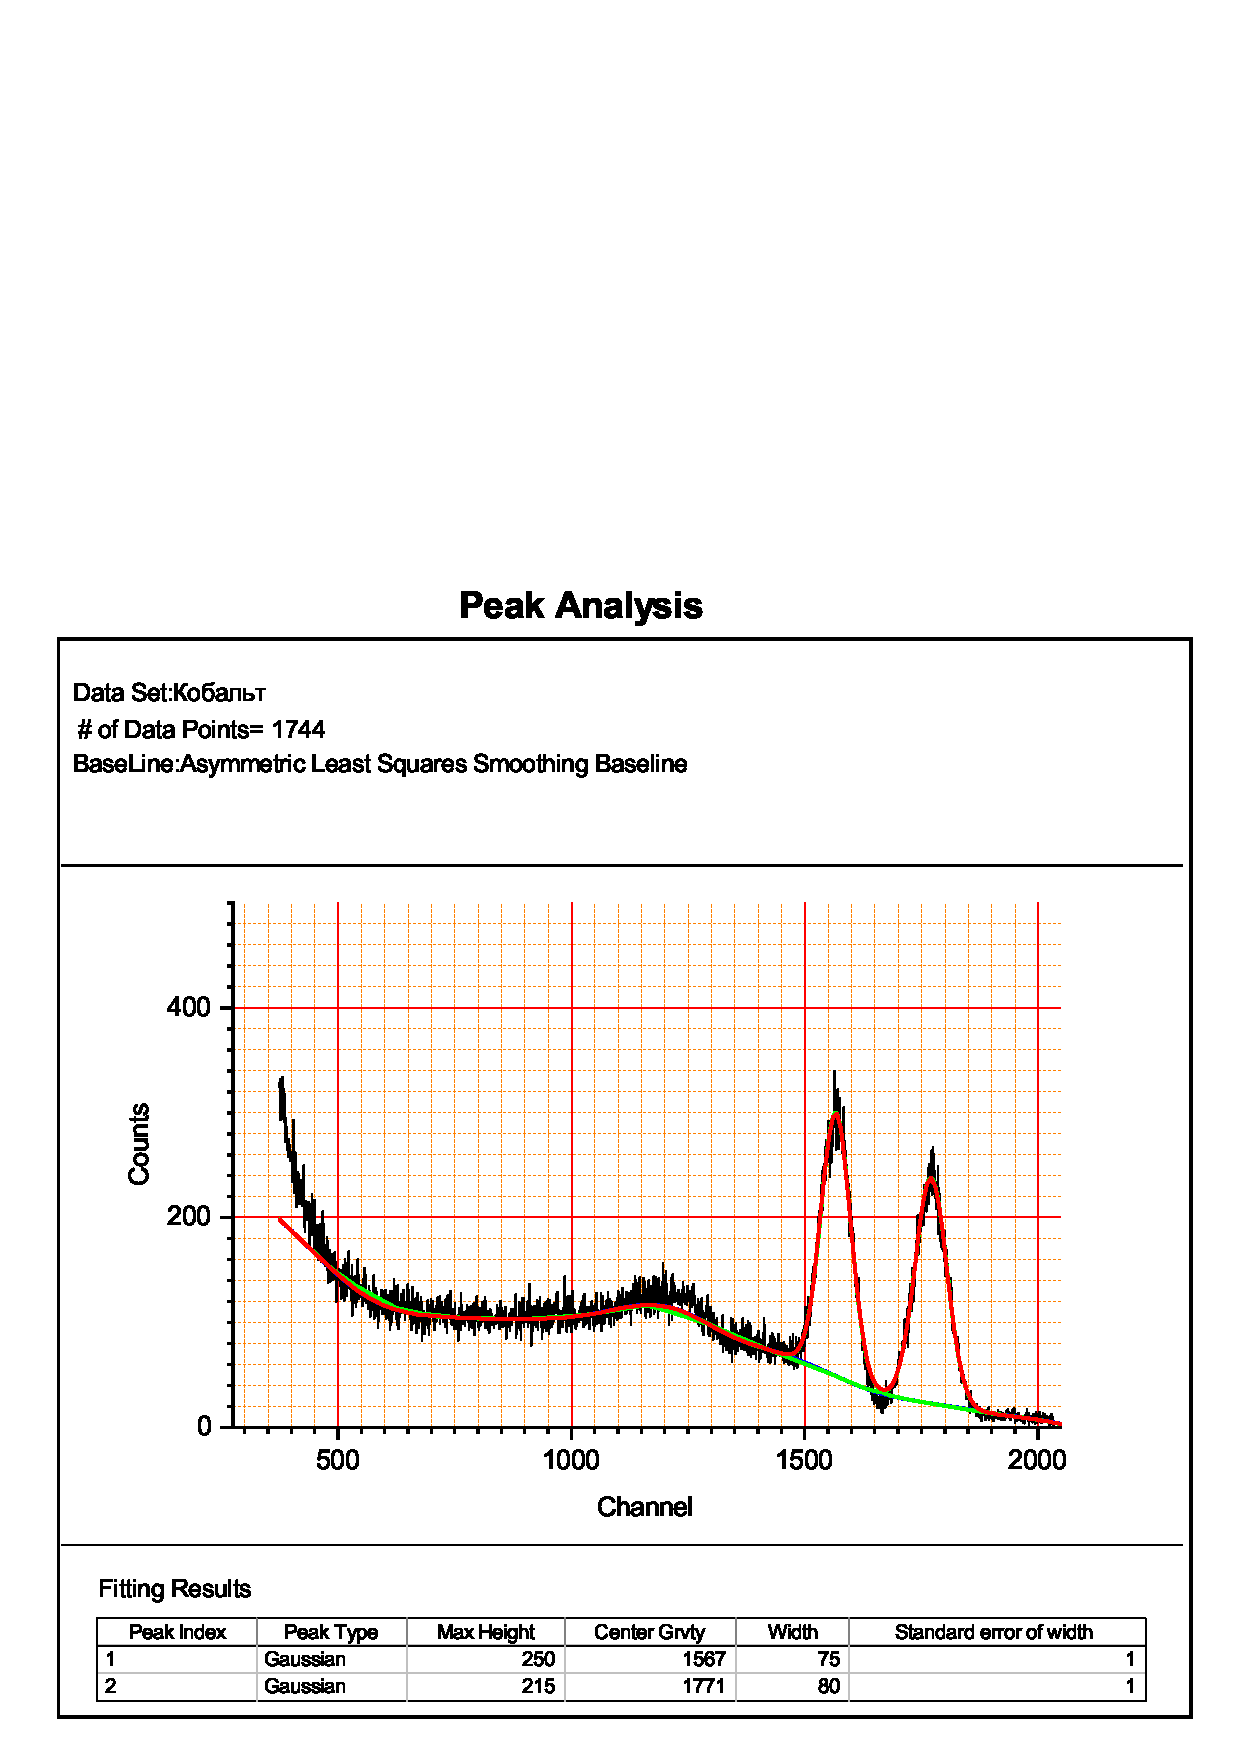
\includegraphics[width=0.6\textwidth]{2.png}
    \caption{Экспериментальная установка}
\end{figure}

\underline{Экспериментальная установка} \newline
\par
Стальная гитарная струна 1 закрепляется в горизонтальном положении между двумя стойками с зажимами 2 и 3, расположенными на массивной станине 4. Один конец струны закреплен в зажиме 2 неподвижно. К противоположному концу струны, перекинутому через блок, прикреплена платформа с грузами 5, создающими натяжение струны. Зажим 3 можно передвигать по станине, устанавливая требуемую длину струны. Возбуждение и регистрация колебаний струны осуществляются с помощью электромагнитных датчиков (вибраторов), расположенных на станине под струной. Электромагнитный датчик 6 подключен к звуковому генератору 7 и служит для возбуждения колебаний струны, частота которых измеряется с помощью частотомера 10 (в некоторых установках частотомер встроен в генератор). Колебания струны регистрируются с помощью электромагнитного датчика 8, сигнал с которого передается на вход осциллографа 9. Разъёмы, через которые датчики с помощью кабелей соединяются с генератором и осциллографом, расположены на корпусе станины.\par

Для регистрации колебаний струны в работе используется электронный осциллограф, соединённый с электромагнитным датчиком 8. Он позволяет регистрировать колебания в случаях, когда это невозможно сделать визуально. Также с помощью осциллографа можно измерять амплитуду возбуждения и форму сигнала, что даёт возможность установить, является ли режим возбуждения стоячих волн линейным, иными словами, имеет ли место прямая пропорциональность между силой возбуждения и амплитудой колебаний струны.
\newpage


\section{Данные}

На экспериментальной установке в зависимости от суммарной массы было сделано 50 измерений частоты от номера гармоники - при 5 разных натяжениях - 10 замеров.
Используемые зависимости:
\[u = \sqrt{\frac{T}{\rho_{l}}}\]
\[\nu_{n} = u \cdot \frac{n}{2L} = \frac{n}{2L}\sqrt{\frac{T}{\rho_{l}}}\]


\begin{itemize}
    \item Длина струны постоянна и равна $L = 50 \text{ см} = 0,5 \text{ м}$ 
    \item Измеряемый диапазон $n \in [1,10]$
    \item Погонная плотность $\rho_{l} = 568,4 \text{ мг/м} = 568,4 \cdot 10^{-6} \text{ кг/м}$
\end{itemize}

\begin{table}[!h]
\begin{tabular}{|l|l|l|l|l|l|}
\hline
                & 1     & 2     & 3   & 4     & 5     \\ \hline
Массы грузов, г & 487,4 & 494,6 & 495 & 419,5 & 491,9 \\ \hline
\end{tabular}
\end{table}

\begin{table}[!h]
\begin{tabular}{|c|ccc|ccc|ccc|ccc|ccc|}
\hline
Опыт                                                     & \multicolumn{3}{c|}{№1}                                                         & \multicolumn{3}{c|}{№2}                                                         & \multicolumn{3}{c|}{№3}                                                         & \multicolumn{3}{c|}{№4}                                                         & \multicolumn{3}{c|}{№5}                                                         \\ \hline
\begin{tabular}[c]{@{}c@{}}Сила\\ натяжения\end{tabular} & \multicolumn{3}{c|}{10,8 Н}                                                  & \multicolumn{3}{c|}{15,64 Н}                                                    & \multicolumn{3}{c|}{20,5 Н}                                                    & \multicolumn{3}{c|}{24,6 Н}                                                    & \multicolumn{3}{c|}{29,42 Н}                                                   \\ \hline
                                                         & \multicolumn{1}{c|}{n}  & \multicolumn{1}{c|}{$\nu_{0}, Гц$} & $\nu_{real}, Гц$ & \multicolumn{1}{c|}{n}  & \multicolumn{1}{c|}{$\nu_{0}, Гц$} & $\nu_{real}, Гц$ & \multicolumn{1}{c|}{n}  & \multicolumn{1}{c|}{$\nu_{0}, Гц$} & $\nu_{real}, Гц$ & \multicolumn{1}{c|}{n}  & \multicolumn{1}{c|}{$\nu_{0}, Гц$} & $\nu_{real}, Гц$ & \multicolumn{1}{c|}{n}  & \multicolumn{1}{c|}{$\nu_{0}, Гц$} & $\nu_{real}, Гц$ \\ \hline
                                                         & \multicolumn{1}{c|}{1}  & \multicolumn{1}{c|}{137,8}         & 136              & \multicolumn{1}{c|}{1}  & \multicolumn{1}{c|}{165,9}         & 163,7            & \multicolumn{1}{c|}{1}  & \multicolumn{1}{c|}{189,9}         & 187              & \multicolumn{1}{c|}{1}  & \multicolumn{1}{c|}{208,1}         & 209              & \multicolumn{1}{c|}{1}  & \multicolumn{1}{c|}{227,5}         & 228,6            \\ \hline
                                                         & \multicolumn{1}{c|}{3}  & \multicolumn{1}{c|}{413,4}         & 410              & \multicolumn{1}{c|}{3}  & \multicolumn{1}{c|}{497,7}         & 493              & \multicolumn{1}{c|}{3}  & \multicolumn{1}{c|}{569,7}         & 563              & \multicolumn{1}{c|}{3}  & \multicolumn{1}{c|}{624,3}         & 630              & \multicolumn{1}{c|}{3}  & \multicolumn{1}{c|}{682,5}         & 687              \\ \hline
                                                         & \multicolumn{1}{c|}{5}  & \multicolumn{1}{c|}{689}           & 685              & \multicolumn{1}{c|}{5}  & \multicolumn{1}{c|}{829,5}         & 824              & \multicolumn{1}{c|}{5}  & \multicolumn{1}{c|}{949,5}         & 940              & \multicolumn{1}{c|}{5}  & \multicolumn{1}{c|}{1040,5}        & 1051             & \multicolumn{1}{c|}{5}  & \multicolumn{1}{c|}{1137,5}        & 1146             \\ \hline
                                                         & \multicolumn{1}{c|}{7}  & \multicolumn{1}{c|}{964,6}         & 965              & \multicolumn{1}{c|}{7}  & \multicolumn{1}{c|}{1161,3}        & 1157             & \multicolumn{1}{c|}{7}  & \multicolumn{1}{c|}{1329,3}        & 1319             & \multicolumn{1}{c|}{7}  & \multicolumn{1}{c|}{1456,7}        & 1474             & \multicolumn{1}{c|}{7}  & \multicolumn{1}{c|}{1592,5}        & 1607             \\ \hline
                                                         & \multicolumn{1}{c|}{9}  & \multicolumn{1}{c|}{1240,2}        & 1247             & \multicolumn{1}{c|}{9}  & \multicolumn{1}{c|}{1493,1}        & 1493             & \multicolumn{1}{c|}{9}  & \multicolumn{1}{c|}{1709,1}        & 1702             & \multicolumn{1}{c|}{9}  & \multicolumn{1}{c|}{1872,9}        & 1899             & \multicolumn{1}{c|}{9}  & \multicolumn{1}{c|}{2047,5}        & 2069             \\ \hline
                                                         & \multicolumn{1}{c|}{2}  & \multicolumn{1}{c|}{275,6}         & 272              & \multicolumn{1}{c|}{2}  & \multicolumn{1}{c|}{331,8}         & 328              & \multicolumn{1}{c|}{2}  & \multicolumn{1}{c|}{379,8}         & 375              & \multicolumn{1}{c|}{2}  & \multicolumn{1}{c|}{416,2}         & 419              & \multicolumn{1}{c|}{2}  & \multicolumn{1}{c|}{455}           & 457              \\ \hline
                                                         & \multicolumn{1}{c|}{4}  & \multicolumn{1}{c|}{551,2}         & 546              & \multicolumn{1}{c|}{4}  & \multicolumn{1}{c|}{663,6}         & 659              & \multicolumn{1}{c|}{4}  & \multicolumn{1}{c|}{759,6}         & 752              & \multicolumn{1}{c|}{4}  & \multicolumn{1}{c|}{832,4}         & 839              & \multicolumn{1}{c|}{4}  & \multicolumn{1}{c|}{910}           & 916              \\ \hline
                                                         & \multicolumn{1}{c|}{6}  & \multicolumn{1}{c|}{826,8}         & 828              & \multicolumn{1}{c|}{6}  & \multicolumn{1}{c|}{995,4}         & 992              & \multicolumn{1}{c|}{6}  & \multicolumn{1}{c|}{1139,4}        & 1130             & \multicolumn{1}{c|}{6}  & \multicolumn{1}{c|}{1248,6}        & 1260             & \multicolumn{1}{c|}{6}  & \multicolumn{1}{c|}{1365}          & 1376             \\ \hline
                                                         & \multicolumn{1}{c|}{8}  & \multicolumn{1}{c|}{1102,4}        & 1105             & \multicolumn{1}{c|}{8}  & \multicolumn{1}{c|}{1327,2}        & 1324             & \multicolumn{1}{c|}{8}  & \multicolumn{1}{c|}{1519,2}        & 1509             & \multicolumn{1}{c|}{8}  & \multicolumn{1}{c|}{1664,8}        & 1685             & \multicolumn{1}{c|}{8}  & \multicolumn{1}{c|}{1820}          & 1837             \\ \hline
                                                         & \multicolumn{1}{c|}{10} & \multicolumn{1}{c|}{1378}          & 1387             & \multicolumn{1}{c|}{10} & \multicolumn{1}{c|}{1659}          & 1662             & \multicolumn{1}{c|}{10} & \multicolumn{1}{c|}{1899}          & 1893             & \multicolumn{1}{c|}{10} & \multicolumn{1}{c|}{2081}          & 2110             & \multicolumn{1}{c|}{10} & \multicolumn{1}{c|}{2275}          & 2301             \\ \hline
\end{tabular}
\end{table}

\section{Обработка данных}
На основе данных эксперимента были построены графики $\nu_{real}(n), \nu_{0}(n)$,реальной частоты от n и расчетной частоты от n.
Для графика 
Получаем что при увеличении натяжения $T$ увеличивается и $u$ и при этом растет разница между рассчитываемыми и реальными значениями u. 

Погрешность образуется из случайной и систематической: погрешность при измерении длины  $\sigma_{L} = 0,0005$, пренебрежем погрешностями генератора частот и осцилографа
\[\text{Среднее значение:  } \overline{u} = \frac{1}{10}\sum\limits_{i=1}^{10} u_{i} \approx 137,4\]
\[\text{Среднеквадратическое отклонение:  } \sigma_{u} = \sqrt{\frac{1}{10}\sum\limits_{i=1}^{10} (u_{i} - \overline{u})^2} \approx 0,97\]
\[\text{Погрешность среднего значения(случайная):  } \sigma_{u}^{\text{случ}} = \frac{\sigma_{u}}{\sqrt{10}} \approx 0,3\]
\[\text{Систематическая погрешность:  }\sigma_{u}^{\text{сист}} = u\sqrt{\left( \frac{du}{dT}\right)^2 \sigma_{T}^2} = u \cdot \sigma_{L} \approx 0,069\]
\[\text{Полная погрешность:  }\sigma_{u}^{\text{полн}} = \sqrt{\sigma_{\text{сист}}^2 + \sigma_{\text{случ}}^2} \approx 0,3\]
Получаем $u = 137,4 \pm 0,3 (\varepsilon_{u} = 0,2\%)$ для натяжения T = 10,8 Н

Аналогично для погонной плотности $\rho_{l}$ получаем:
\[\text{Среднее значение:  } \overline{\rho} = \frac{1}{10}\sum\limits_{i=1}^{10} \rho_{i} \approx 567,9\]
\[\text{Среднеквадратическое отклонение:  } \sigma_{\rho} = \sqrt{\frac{1}{10}\sum\limits_{i=1}^{10} (\rho_{i} - \overline{\rho})^2} \approx 0,64\]
\[\text{Погрешность среднего значения(случайная):  } \sigma_{\rho}^{\text{случ}} = \frac{\sigma_{\rho}}{\sqrt{5}} \approx 0,36\]
\[\text{Систематическая погрешность:  }\sigma_{\rho}^{\text{сист}} = \rho\sqrt{\left( \frac{d\rho}{du}\right)^2 \sigma_{u}^2} = \rho \cdot 2\sigma_{u}\approx 2,3\]
\[\text{Полная погрешность:  }\sigma_{\rho}^{\text{полн}} = \sqrt{\sigma_{\text{сист}}^2 + \sigma_{\text{случ}}^2} \approx 2,33\]
Получаем $\rho_{l} = 567,9 \pm 2,33 (\varepsilon_{\rho} = 0,4\%)$

\section{Выводы}

В данной работе были исследованы колебания поперечных волн на примере струны. 

Были построенны графики зависимостей $\nu(n)$ и $u^2(T)$, благодаря которыми были экспериментально доказаны формулы зависимости частоты от номера гармоники. Также была измерена экспериментально погонная плотность с высокой точностью, что показывает точность установки и корректнось эксперимента.

\newpage

\begin{figure}[t]
    \centering
    \includegraphics[width=1\textwidth]{graphic1.png}
    \caption{Зависимость $\nu_{real}(n)$ реальной частоты от номера n гармоники с аппроксимирующими прямыми для 5 разных натяжений}
\end{figure}

\begin{figure}[t]
    \centering
    \includegraphics[width=1\textwidth]{graphic2.png}
    \caption{Зависимость $u^2(T)$ и расчет погонной плотности $\rho_{l}$}
\end{figure}
\end{document}
